\documentclass{beamer}
\usepackage[english]{layout}
\usepackage[utf8]{inputenc}
\usepackage[english]{babel}
\usepackage[T1]{fontenc}
\usepackage{amsmath, soul, color, multicol, type1cm, verbatim, latexsym, dsfont, float, listings,alltt,graphicx}
\usepackage[export]{adjustbox}
\usepackage[caption = false]{subfig}
%\usepackage[demo]{graphicx}
\usepackage[official]{eurosym}
\usepackage{beamerthemesplit}
\usetheme{Frankfurt}
\usecolortheme{lily}
%\usefonttheme{structuresmallcapsserif}
\usefonttheme{professionalfonts}
\setbeamercovered{transparent}

%NeSI Colors <---------------------------------------------------------------------------------------
\usecolortheme[RGB={47, 68, 71}]{structure} 
\definecolor{nesidark}{HTML}{2F4447}
\definecolor{nesilight}{HTML}{CED9DF}
\definecolor{nesigrey}{gray}{0.7}
\definecolor{nesilightgrey}{gray}{0.98}
\definecolor{nesidarkgrey}{gray}{0.3}
\definecolor{nesiblue}{HTML}{2B9FC2}
\setbeamercolor{block title}{fg=black,bg=nesigrey}
\setbeamercolor{block body}{bg=nesilightgrey,fg=nesidarkgrey}
\setbeamercolor{block body alerted}{bg=white,fg=black}
\setbeamercolor{alerted text}{bg=white,fg=black}
%NeSI Custom Code Hightlight <---------------------------------------------------------------------------------------
\lstdefinestyle{customcode}{
  belowcaptionskip=1\baselineskip,
  breaklines=true,
  xleftmargin=\parindent,
  showstringspaces=false,
  basicstyle=\ttfamily,
  keywordstyle=\bfseries\color{green!40!black},
  commentstyle=\itshape\color{purple!40!black},
  identifierstyle=\color{blue},
  stringstyle=\color{orange},
}
%NeSI template customization
%\setbeamerfont{title}{size=\huge}
\frenchspacing
\hyphenation{NeSI}
\newcommand\BackgroundPicture[1]{%
\setbeamertemplate{background}{%
\parbox[c][\paperheight]{\paperwidth}{%
\vfill \hfill \includegraphics[height=0.9\paperheight]{#1}
\hfill \vfill
}}}
\setbeamertemplate{blocks}[default]%[shadow=false]
\useinnertheme{circles}
\setbeamertemplate{title page}[default][center,rounded=false,shadow=false]
%TITLE <---------------------------------------------------------------------------------------
\title{MIGRATE: a case study of optimizing of an open source application for estimation of population sizes and gene flow}
%\subtitle{Computational Science Team @ NeSI}
\author{Jordi Blasco (jordi.blasco@nesi.org.nz)\\Sarah Knight (s.knight@auckland.ac.nz)}
\date{}

\begin{document}

{
\setbeamertemplate{background canvas}{
\includegraphics[height=0.99\paperheight]{NeSI_img/Slide00.png}} 
\begin{frame}[plain]
\vspace{1cm}
\titlepage
\end{frame}
}

%\BackgroundPicture{NeSI_img/SlideXX.png}
\begin{frame}
\frametitle{Outline}
\begin{multicols}{2}
   \tableofcontents
 \end{multicols}
 \end{frame}
%%%%%%%%%%%%%%%%%%%%%%%%%%%%%%%%%%%%%%%%%%%%%%%%%%%%%%%%%%%%%%%%%%%%%%%%%%%%%%%%%%%%%%%%%%%%%%%
%%%%%%%%%%%%%%%%%%%%%%%%%%%%%%%%%%%%%%%%%%%%%%%%%%%%%%%%%%%%%%%%%%%%%%%%%%%%%%%%%%%%%%%%%%%%%%%

\section{Science Background}
\subsection{}
%Sarah Knight research
\frame[t]
{
  \frametitle{Science Background}
 \begin{block}{Estimating migration rates in the budding yeast}
%Eukaryotic microbes are key ecosystem drivers, but we have little theory and few data elucidating the processes influencing their observed population patterns.

%Because of their large population sizes, and ease of transfer, one might expect microbial populations to be well mixed, but 
There is increasing evidence showing that \textbf{microbial populations} are not homogeneous but \textbf{structured}. 

The processes that drive population structure and connectivity have \textbf{implications} for \textbf{understanding} the \textbf{evolutionary trajectories} of these organisms.
 \end{block}
  \begin{block}{Yeast is of significant commercial importance}
Yeast plays a \textbf{key role} in the production of \textbf{bread}, \textbf{wine}, \textbf{beer} and other \textbf{alcoholic} beverages and is also widely used by the scientific community as a \textbf{model research} organism. 

%While we have a vast knowledge of its cell biology, genetics and increasingly its ecology and evolution, studies of its population patterns are often confounded by geography.

 \end{block}
}

\frame[t]
{
  \frametitle{Science Background}
 \begin{block}{Regions and analyses of population structure and connectivity}
 Since microbes are inherently difficult to observe directly, the study relies on \textbf{genetic methods to infer their movements}.
 
\textbf{Samples} were \textbf{collected} form vineyards and surrounding native bush in major \textbf{Sauvignon Blanc} growing \textbf{regions}. The samples were genotyped in \textbf{850 individual} isolates at \textbf{eight} \textbf{microsatellite} \textbf{loci}\footnote{Locus (plural loci) is the specific location of a gene, DNA sequence, or position on a chromosome.}.
  \end{block}
}

\frame[t]
{
  %\frametitle{Science Background}
\begin{center}
 \vspace*{-0.2cm}
 \begin{figure}
 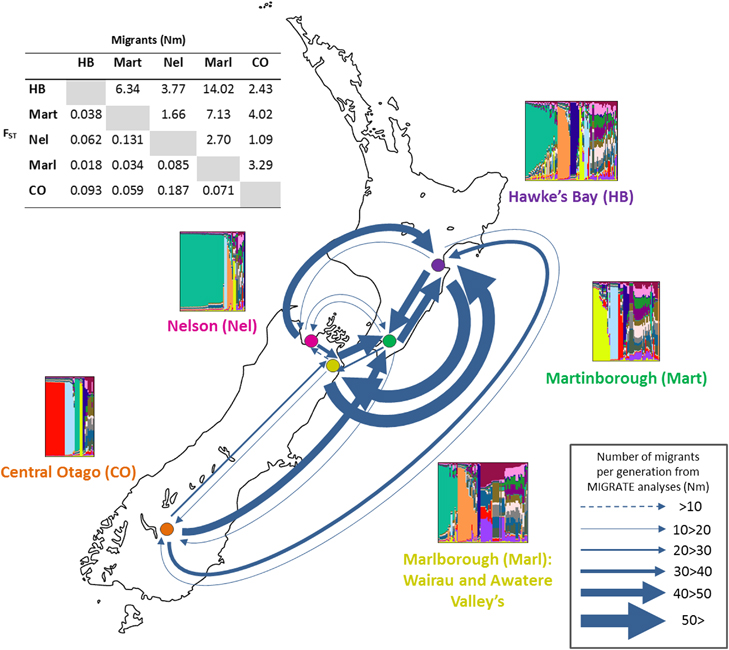
\includegraphics[width=0.7\textwidth]{NeSI_img/ismej2014132f1.jpg}
 \vspace*{-0.1cm}
 \caption{Source : Knight, S. and Goddard, M. R. (2014). Quantifying separation and similarity in a Saccharomyces cerevisiae metapopulation. ISME J. DOI: 10.1038/ismej.2014.132.}
 \end{figure}
\end{center}
}


\section{Computational Needs}
\subsection{Dimension of the Problem}
\frame[t]
{
  \frametitle{Dimension of the Problem}
 \begin{block}{Evaluating Size Magnitude and Computational Requirements}
 The dataset was used to infer patterns of population structure and connectivity between these regions and between managed and unmanaged ecosystems within each region.
 \begin{itemize}
     \item \textbf{Analyses} of genetic data \textbf{to infer migration rates} are typically very \textbf{computationally} \textbf{expensive}.
     \item The final dataset comprised \textbf{369 microsatellite profiles}. 
     \item \textbf{Bayesian coalescent} approach implemented in \textbf{MIGRATE} (Beerli, 2006; Beerli, 2009) had been used.
     \item \textbf{Final run composed of ten replicate MCMC\footnote{Markov chain Monte Carlo} chains of one million steps in length across all eight loci.}
 \end{itemize}

\end{block}
}
 
\subsection{Domain Decomposition}
\frame[t]
{
  \frametitle{Domain Decomposition Strategy}
\begin{block}{Independence of loci}
\begin{itemize}
    \item \textbf{Collected loci} are considered \textbf{unlinked}, which implies that \textbf{each locus} has a \textbf{different coalescent history}.
    \item Each locus can then be run independently from each other.
    %\item If the loci are a few 10,000 bases apart then because of recombination the independence assumptions works quite well.
    \item Independent runs are combined in a maximum likelihood context by multiplying the likelihood curves.
    \item The replication option allows to replicate each locus. 
    \item Bayesian inference will run the analysis $n$ times and combine the collected MCMC samples.
    \item Maximum likelihood (ML) analysis allows combination of independent replicates. 
\end{itemize}
\end{block}
}


\frame[t]
{
  \frametitle{Parallel approach for Domain Decomposition}
% \begin{block}{Parallel approach for Domain Decomposition}
 \vspace*{-0.5cm}
 \begin{figure}
 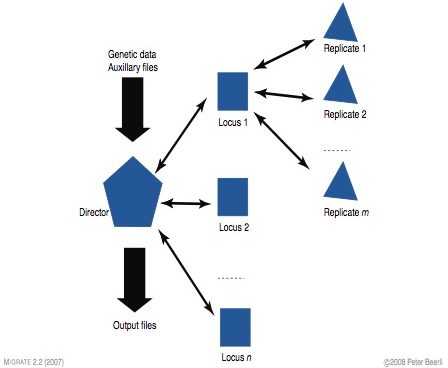
\includegraphics[width=0.8\textwidth]{NeSI_img/domain_decomposition.png}
 \vspace*{-0.3cm}
 \caption{Source : http://popgen.sc.fsu.edu/Migrate}
 \end{figure}
% \end{block}
}


\frame[t]
{
  \frametitle{Domain Decomposition}
\begin{block}{Improving Parallel Jobs Efficiency}
\begin{itemize}
%\item For complex problems with many loci it may help to have 10 or more replications because each MCMC chain will explore slightly different solution spaces.
\item The runtimes are rather different for each node and the director node will wait for the slowest node.
\item In order to improve the usage of HPC resources it is better to allocate fewer nodes than (loci * replicates).
\item Running the same problem on less nodes will definitely increase the runtime but also the efficiency.
%\item Running the same problem on 11 nodes instead of 51 will increase the runtime perhaps by a factor of 2 but reduce the resources by 5.
%The only problems with replicates is that we need to make sure that the MCMC chain has converged in the burn-in, this will need large burn-in in because the only few samples are taken for each replicate. Since we do not know how long a particular run goes, I often experiment by changing the default parameters for trials run. For example instead of using the increment between collected samples (long-inc) of a 100 (default), I set it to 1, 
\end{itemize}
\end{block}
}



\frame[t]
{
  \frametitle{Parallel approach for Domain Decomposition}
 \vspace*{-1.8cm}
 \hspace*{-2cm}
 \begin{figure}
 \subfloat[51  cores]{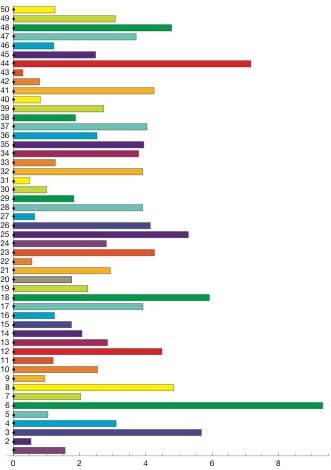
\includegraphics[width=0.4\textwidth]{NeSI_img/shapeimage_1.jpg}}
 \subfloat[11  cores]{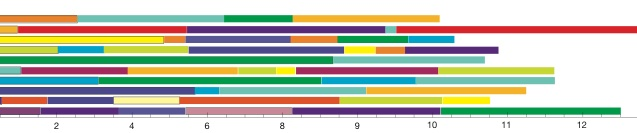
\includegraphics[width=0.7\textwidth]{NeSI_img/shapeimage_2.jpg}}
 \vspace*{-0.2cm}
 \caption{Source : http://popgen.sc.fsu.edu/Migrate}
 \end{figure}
}


\section{Application Performance Analysis}
\frame[t]
{
  \frametitle{Application Performance Analysis}
\begin{block}{Benchmark details}
Sarah Knight provided a representative short test to be used as benchmark, based on real data.
\begin{itemize}
\item long-chains=1
\item long-inc=1
\item long-sample=30000
\item burn-in=1000
\item auto-tune=YES:0.440000
\item replicate=YES:95
\end{itemize}
Very short walltime (around two minutes using 160 cores).
\end{block}
}

%\subsection{Pan Cluster Configuration}
\subsection{Processor Generations}

\frame[t]
{
  \frametitle{Application Performance Analysis}
\begin{block}{Processor Generations}
System components used:\\ 
\begin{multicols}{2}
\textbf{Westmere}
\begin{itemize}
\item Intel X5660@2.8GHz
\item 2-socket 6-core
\item 2x QPI 6.4 GT/s
\item 1333MHz DDR3
\item 96GB RAM
\item Mellanox Connect-IB QDR
\item SSE4 (Streaming SIMD Extensions 4)
\end{itemize}
\textbf{SandyBridge}
\begin{itemize}
\item Intel E5-2680@2.7GHz
\item 2-socket 8-core
\item 2x QPI 8 GT/s
\item 1600MHz DDR3
\item 128GB RAM
\item Mellanox ConnectX-3 QDR
\item Advanced Vector Extensions (AVX)
\end{itemize}
\end{multicols}
\end{block}
}

\frame[t]
{
  \frametitle{Application Performance Analysis}
\begin{block}{Processor Generations}
Intel E5-2680 Series outperforms prior generation. Up to 36\% higher performance than Intel X5660 using 144 cores.
\begin{center}
 \vspace*{-0.2cm}
 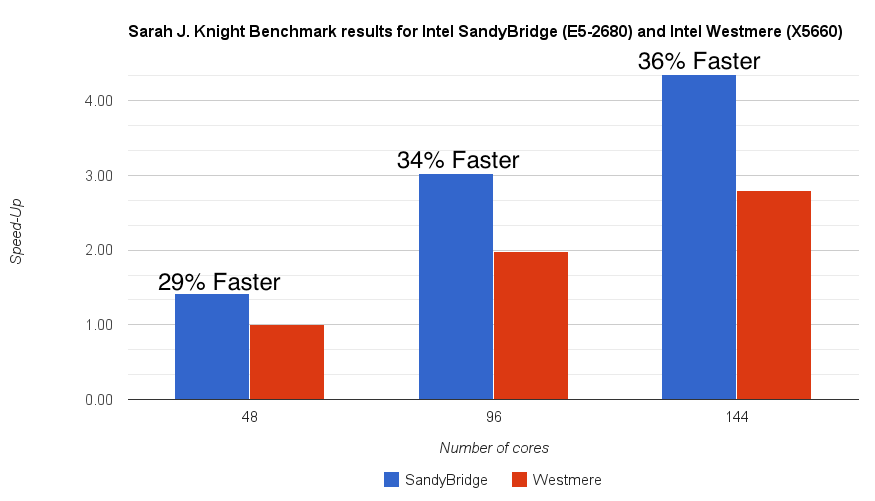
\includegraphics[width=0.9\textwidth]{NeSI_img/migrate-hardware-speedup.png}
\end{center}
\end{block}
}



\subsection{Compilers}
\frame[t]
{
  \frametitle{Application Performance Analysis}
\begin{block}{Compilers}
\begin{itemize}
    \item Using \textbf{Intel Composer XE 2013 SP1} compiler shows best performance
    \item Up to \textbf{x2.14 better performance} than compiling MIGRATE using BLACS (0.2.8), FFTW(3.3.4), GCC(4.8.2), OpenBLAS(0.2.8), OpenMPI(1.6.5), ScaLAPACK(2.0.2).
    \item Instability in the performance observed while running code compiled with GNU toolchain.
     \item \textbf{Tuned version bumps} the \textbf{performance} an additional \textbf{19\%} over best value (default options), x2.54 compared with GNU toolchain version.
\end{itemize}
\end{block}
}


\frame[t]
{
  \frametitle{Application Performance Analysis}
\begin{block}{Toolchains Speed-Up}
\begin{center}
 \vspace*{-0.4cm}
 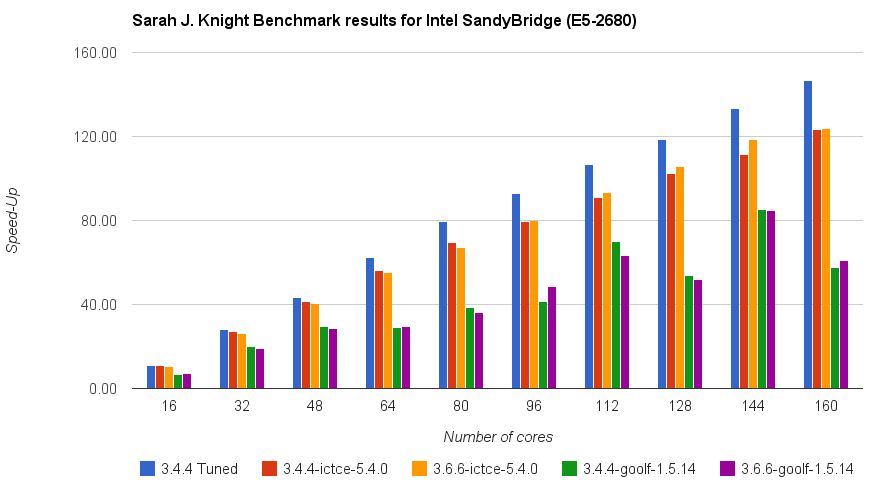
\includegraphics[width=\textwidth]{NeSI_img/migrate-toolchains-speedup.png}
\end{center}
\end{block}
}

\frame[t]
{
  \frametitle{Application Performance Analysis}
\begin{block}{Toolchains Efficiency}
\begin{center}
 \vspace*{-0.4cm}
 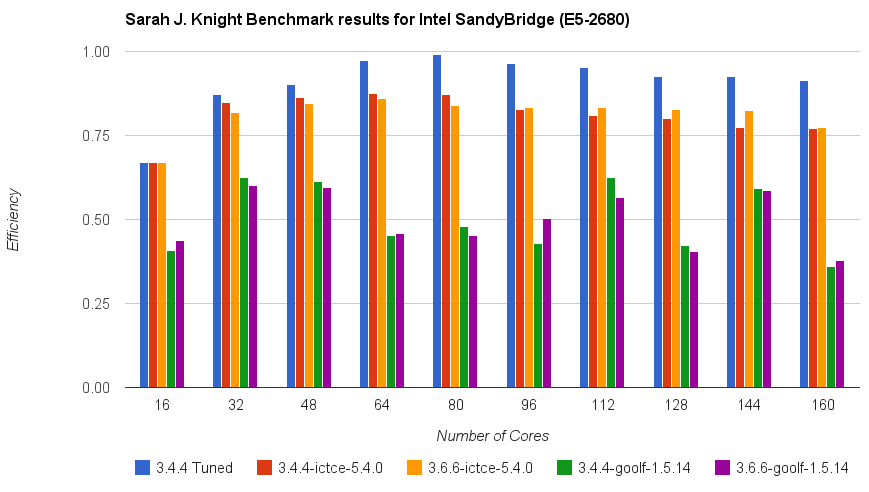
\includegraphics[width=\textwidth]{NeSI_img/migrate-toolchains-efficiency.png}
\end{center}
\end{block}
}


\subsection{MPI Implementations}
\begin{frame}[fragile]
  \frametitle{Application Performance Analysis}
\begin{block}{MPI Implementations and Options}
\begin{itemize}
    \item Intel MPI performs better than OpenMPI as the job grows in number of cores or the problem scales.
    %\item \verb|I_MPI_ADJUST_REDUCE_SCATTER| introduces stability in the MPI communication.
    \item \verb|I_MPI_FABRICS=shm:dapl| fabrics shows some benefits over MLNX OFED for large number of cores.
    \item \verb|I_MPI_WAIT_MODE=enable| processes that waits for receiving messages without polling of the fabric can save CPU time.
    \item \verb|I_MPI_SHM_BYPASS=enable| Turn on/off the intra-node communication mode through network fabric along with shm.
    \item \verb|I_MPI_SHM_CACHE_BYPASS_THRESHOLDS| Set the message copying algorithm threshold for shm device.
    \item \verb|I_MPI_INTRANODE_EAGER_THRESHOLD| Change the eager message size threshold for intra-node communication mode.
\end{itemize}
\end{block}
\end{frame} 
% Options used 
% export I_MPI_FABRICS=shm:dapl
% export I_MPI_FALLBACK=disable
% export I_MPI_DAPL_UD=enable
% export I_MPI_DAPL_SCALABLE_PROGRESS=1
% export I_MPI_PIN_PROCESSOR_LIST='grain=cache2,shift=sock'
% export I_MPI_WAIT_MODE=enable
% export I_MPI_SHM_BYPASS=enable
% export I_MPI_INTRANODE_EAGER_THRESHOLD=262144
% export I_MPI_SHM_CACHE_BYPASS_THRESHOLDS=16384,16384,-1,16384,-1,16384


\subsection{Time Spent by MPI Calls}
\frame[t]
{
  \frametitle{Application Performance Analysis}
\begin{block}{Communication overhead}
$$
T=\frac{MessageSize}{BW}+L
$$
\end{block}
\begin{block}{Time Spent by MPI Calls}
Due to the nature of the code, the major time spent by MPI calls is due to \textbf{MPI\_Recv}.
 \vspace*{-0.6cm}
\begin{figure}[c]
\subfloat[48  cores]{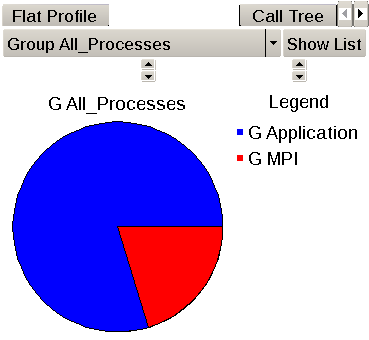
\includegraphics[width = 0.24\textwidth]{NeSI_img/traces-pie-48.png}} 
\subfloat[80  cores]{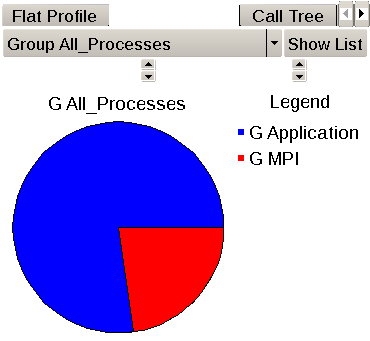
\includegraphics[width = 0.24\textwidth]{NeSI_img/traces-pie-80.png}}
\subfloat[128 cores]{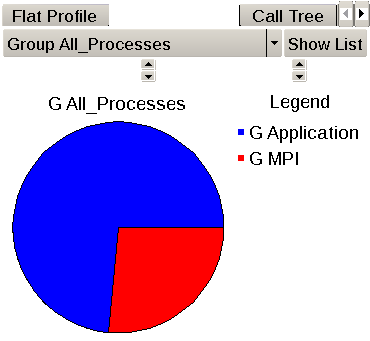
\includegraphics[width = 0.24\textwidth]{NeSI_img/traces-pie-128.png}}
\subfloat[160 cores]{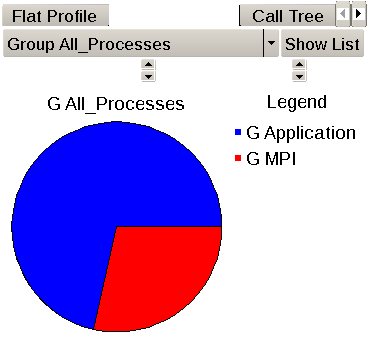
\includegraphics[width = 0.24\textwidth]{NeSI_img/traces-pie-160.png}} 
%\caption{Add your own figures before compiling}
\end{figure}
\end{block}
}

\begin{frame}[fragile]
  \frametitle{Application Performance Analysis}
\begin{block}{Time Spent by MPI Calls - Quantitative View}
\vspace*{-0.5cm}
\begin{figure}
\subfloat[48  cores]{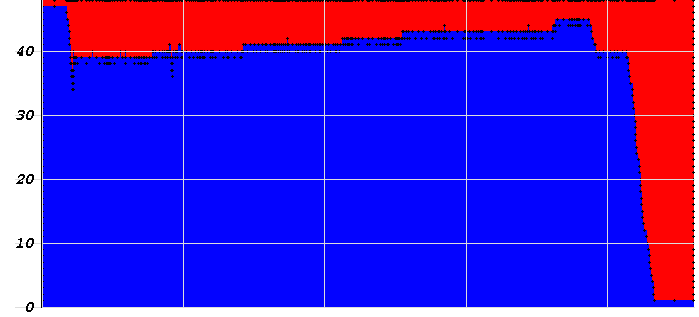
\includegraphics[width = 0.45\textwidth]{NeSI_img/traces-48.png}} 
\subfloat[80  cores]{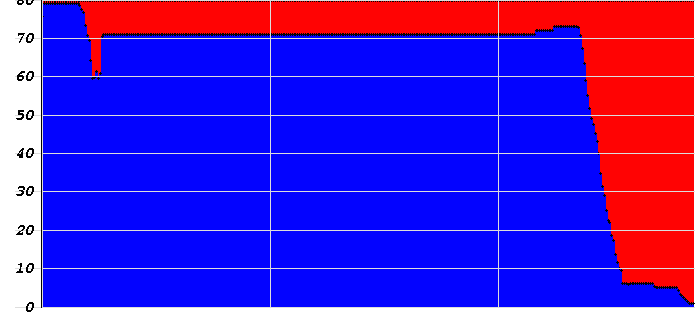
\includegraphics[width = 0.45\textwidth]{NeSI_img/traces-80.png}}\\ 
\vspace*{-0.2cm}
\subfloat[128 cores]{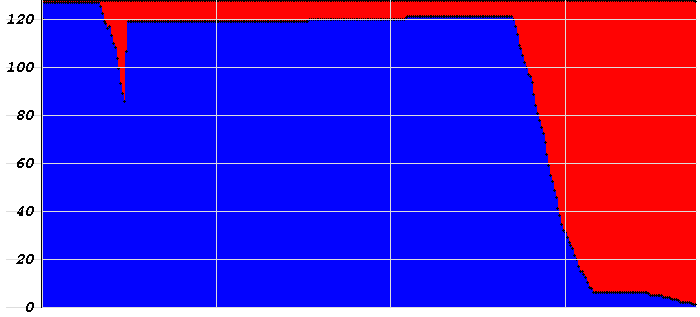
\includegraphics[width = 0.45\textwidth]{NeSI_img/traces-128.png}}
\subfloat[160 cores]{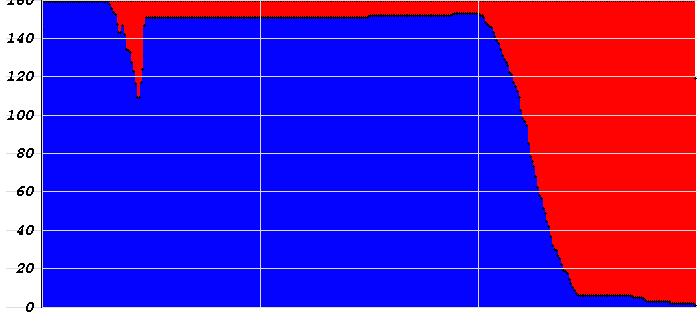
\includegraphics[width = 0.45\textwidth]{NeSI_img/traces-160.png}} 
\vspace*{-0.2cm}
\caption{Number of MPI tasks (y-axis) vs runtime (x-axis). Time spent in MPI (red) grows more than time spent in the application (blue) as the allocation grows.}
\end{figure}
\end{block}
\end{frame} 

\begin{frame}[fragile]
  \frametitle{Application Performance Analysis}
\begin{block}{Time Spent by MPI Calls - Breakdown View}
\vspace*{-0.2cm}
\begin{figure}
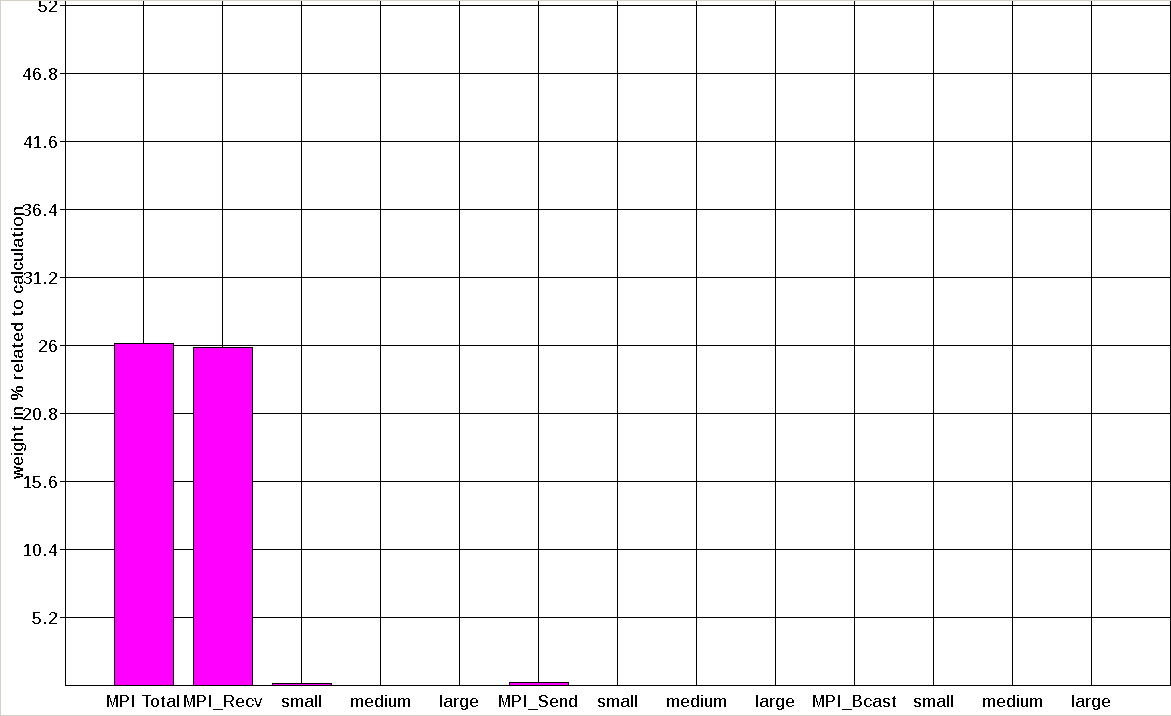
\includegraphics[width = 0.8\textwidth]{NeSI_img/time_mpi_calls_breakdown.png}
\vspace*{-0.2cm}
\caption{Time Spent by MPI Calls using 80 cores.\textbf{MPI\_Recv} is the most expensive operation in this case.}
\end{figure}
\end{block}
\end{frame} 

\subsection{Number of MPI Calls}
\begin{frame}[fragile]
  \frametitle{Application Performance Analysis}
\begin{block}{Number of MPI Calls}
\begin{itemize}
    \item Communication pattern changes as the allocation or the problem scales.
    \item MIGRATE shows a large number of MPI calls for data communications in the final stage.
    \item \textbf{This number grows dramatically if the number of cores is increased while maintaining the problem size.}
\end{itemize}
\end{block}
\end{frame} 


%\begin{frame}[fragile]
%   \frametitle{Application Performance Analysis}
% \begin{block}{Number of MPI Calls}
% \vspace*{-0.4cm}
% \begin{figure}
% \subfloat[48  cores]{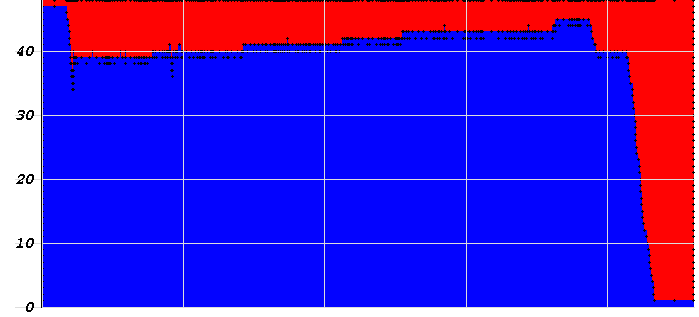
\includegraphics[width = 0.45\textwidth]{NeSI_img/traces-48.png}} 
% \subfloat[80  cores]{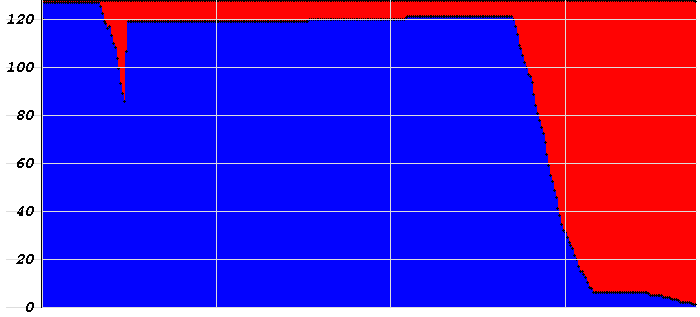
\includegraphics[width = 0.45\textwidth]{NeSI_img/traces-128.png}}\\
% \subfloat[128 cores]{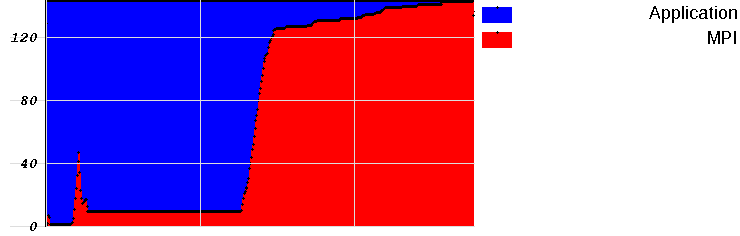
\includegraphics[width = 0.45\textwidth]{NeSI_img/traces-144.png}}
% \subfloat[160 cores]{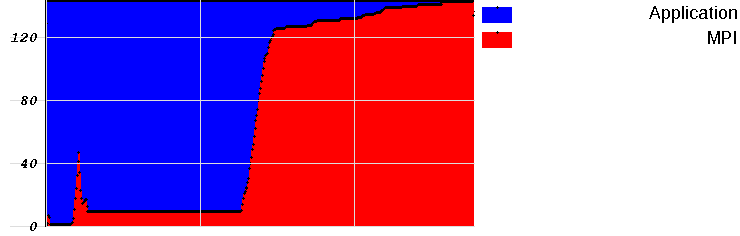
\includegraphics[width = 0.45\textwidth]{NeSI_img/traces-144.png}} 
% %\caption{Add your own figures before compiling}
% \label{some example}
% \end{figure}
% \end{block}
% \end{frame} 



% \subsection{MPI Message Sizes}
% \frame[t]
% {
%   \frametitle{Application Performance Analysis}
% \begin{block}{MPI Message Sizes}
% The amount of data being transferred on number of cores.
% \begin{center}
%  \vspace*{-0.4cm}
%  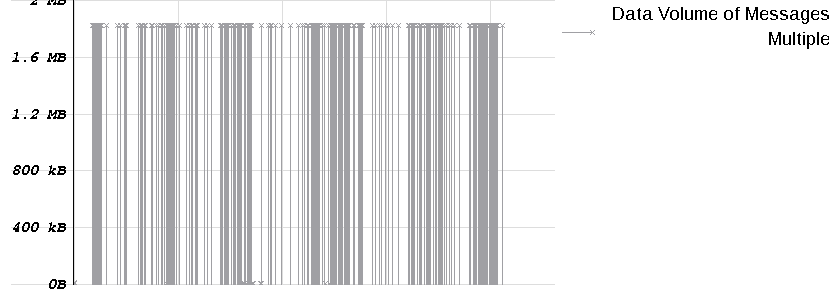
\includegraphics[width=0.6\textwidth]{NeSI_img/data-volume-of-messages-48.png}
%  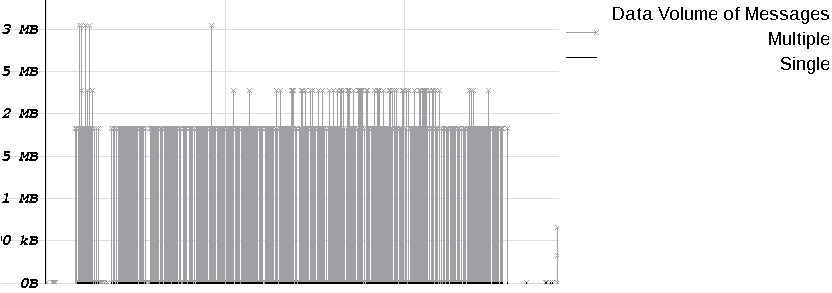
\includegraphics[width=0.6\textwidth]{NeSI_img/data-volume-of-messages-80.png}
% \\
%  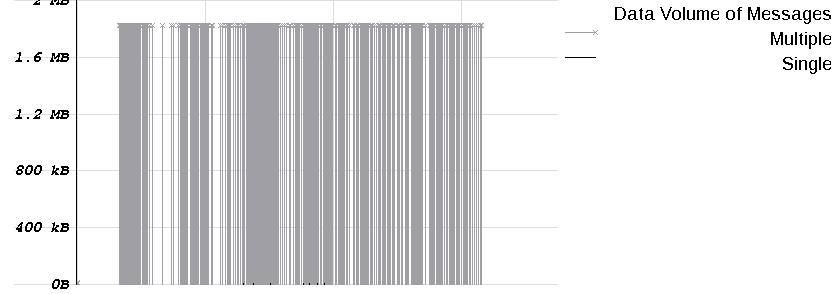
\includegraphics[width=0.6\textwidth]{NeSI_img/data-volume-of-messages-128.png}
%  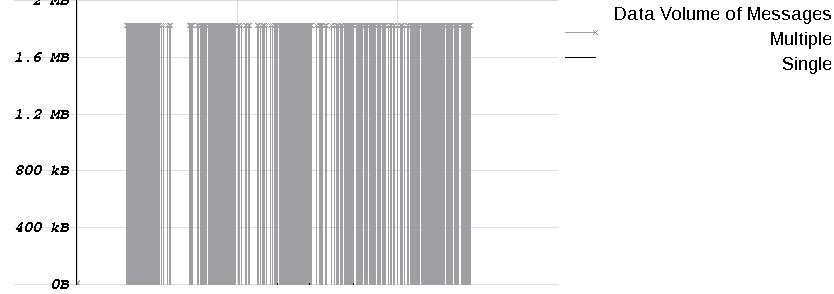
\includegraphics[width=0.6\textwidth]{NeSI_img/data-volume-of-messages-160.png}
% \end{center}
% \end{block}
% }


\subsection{Final Analysis Outcome}
\frame[t]
{
  \frametitle{Final Analysis Outcome}
     \begin{block}{Importance of Performance Analysis}
 \begin{itemize}
 % steep 0 is to understand how the application actually works!
 \item There are theoretical limits but the reality can be really surprising!
 \item The benchmarks can help to discover the real scalability limits.
 \item With this information you can get the results even faster and save computational resources for other jobs.
 \item Intel toolchain definitely improves the performance.
 \item The code can take advantage of new instruction set available in SandyBridge.
 \item Intel Trace Analyzer helped to find most suitable values for Intel MPI.
 \end{itemize}
  \end{block}
}

\frame[t]
{
  \frametitle{Application Performance Analysis}
\begin{block}{Major impact in the efficiency and walltime}
Thanks to the Application Performance Analysis we have been able to reduce significantly the runtime and improve the efficiency.
\end{block}
}

\frame[t]
{
  \frametitle{Application Performance Analysis}
%\begin{block}{Major impact in the efficiency and walltime}
\begin{center}
\vspace*{+2.5cm}
\Huge{From the original version...}
\end{center}
%\end{block}
}

\frame[t]
{
  \frametitle{Application Performance Analysis}
%\begin{block}{Major impact in the efficiency and walltime}
 \vspace*{+1.3cm}
\begin{figure}
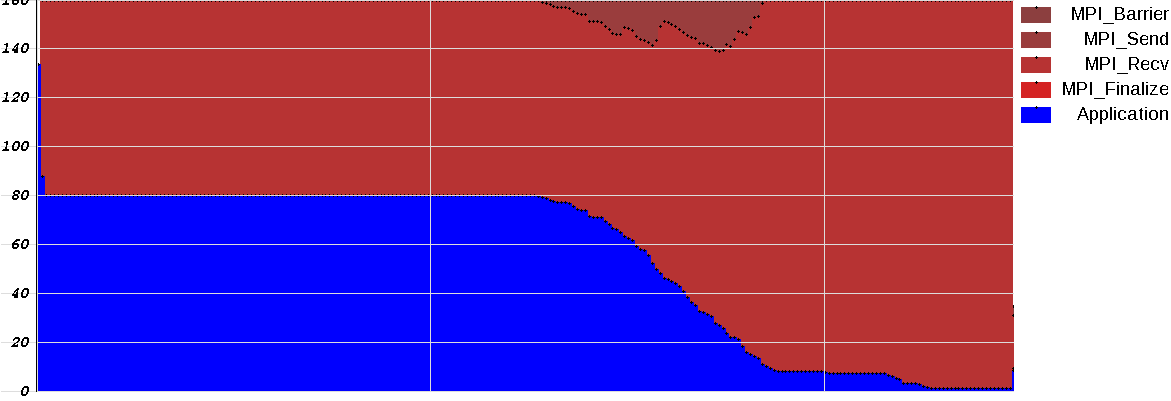
\includegraphics[width=\textwidth]{NeSI_img/comparative-trace-bad.png}
\vspace*{-0.2cm}
\caption{Time spent by MPI calls (red) using 160 cores versus time spent by application (blue). Efficiency $\approx 38\%$}
\end{figure}
%\end{block}
}

\frame[t]
{
  \frametitle{Application Performance Analysis}
%\begin{block}{Major impact in the efficiency and walltime}
\begin{center}
\vspace*{+2.5cm}
\Huge{... to the production one}
\end{center}
%\end{block}
}

\frame[t]
{
  \frametitle{Application Performance Analysis}
%\begin{block}{Major impact in the efficiency and walltime}
 %\vspace*{+1.3cm}
\begin{figure}
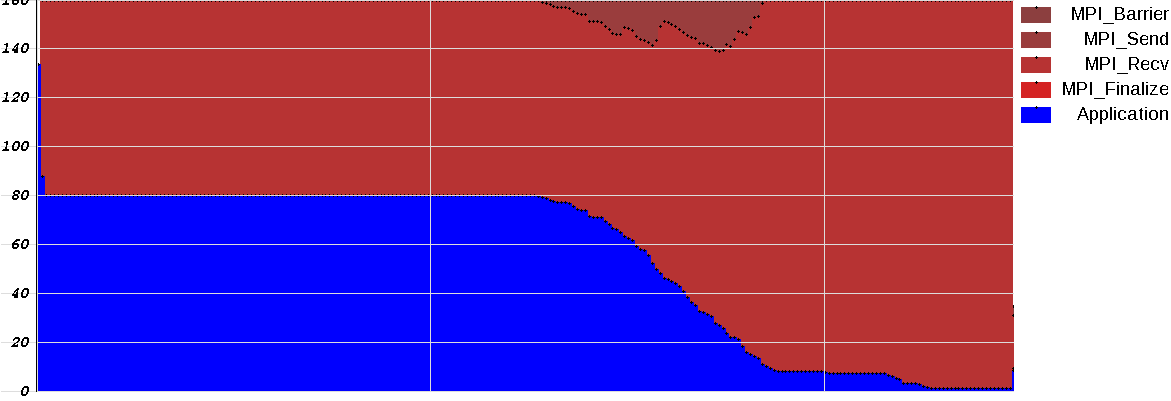
\includegraphics[width=0.3\textwidth,right]{NeSI_img/comparative-trace-bad.png}\\ 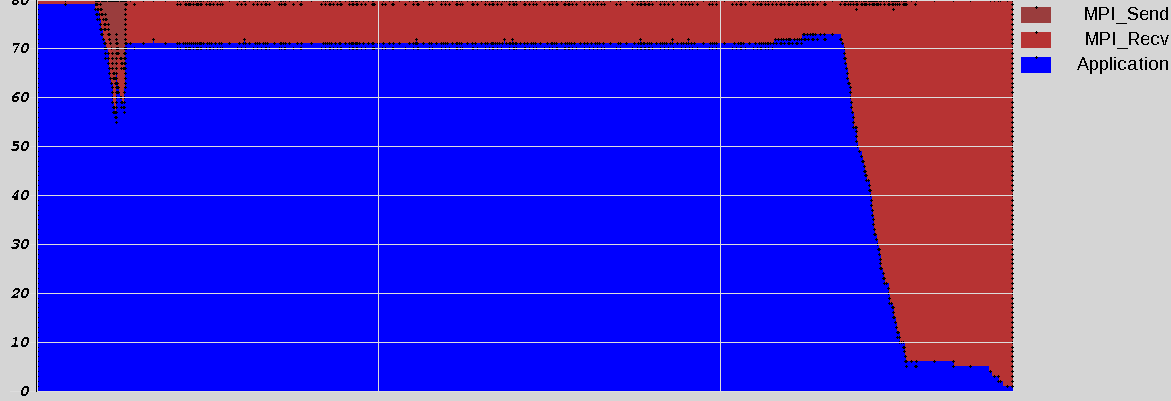
\includegraphics[width=\textwidth]{NeSI_img/comparative-trace-good.png}
\vspace*{-0.2cm}
\caption{Time spent by MPI calls (red) using 80 cores versus time spent by application (blue). Efficiency $\approx 77\%$}
\end{figure}
%\end{block}
}

\frame[t]
{
  \frametitle{Final Analysis Outcome}
  \begin{block}{Researcher Feedback}
\textit{"\textbf{With the help of staff at NeSI}, optimal settings were determined and we managed to run each chain for each locus in parallel, essentially \textbf{reducing the time it took to run the analysis by 80 times!} Even then the analysis still took weeks to run and without the resources provided by NeSI this analysis would not have been possible."} -- Dr. Sarah Knight (UoA)

\includegraphics[width=\textwidth,center]{NeSI_img/logo-ismej.png}\\
Knight, S. and Goddard, M. R. (2014). Quantifying separation and similarity in a Saccharomyces cerevisiae metapopulation. ISME J. DOI: 10.1038/ismej.2014.132. \url{http://www.nature.com/ismej/journal/v9/n2/full/ismej2014132a.html}
  \end{block}

}


{
\setbeamertemplate{background canvas}{
\includegraphics[height=0.99\paperheight]{NeSI_img/Slide00.png}} 
\begin{frame}[plain]
\begin{center}
{\Huge Questions \& Answers}
\end{center}
\end{frame}
}


\end{document}